
\documentclass[MAIN.tex]{subfiles} 
\begin{document} 
\begin{frame}
\begin{figure}
\centering
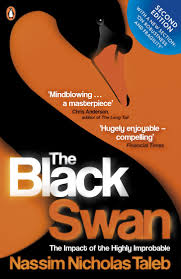
\includegraphics[width=0.5\linewidth]{images/blackswan}

\end{figure}

\end{frame}
%================================================================================ %
	\begin{frame}

\begin{figure}
\centering
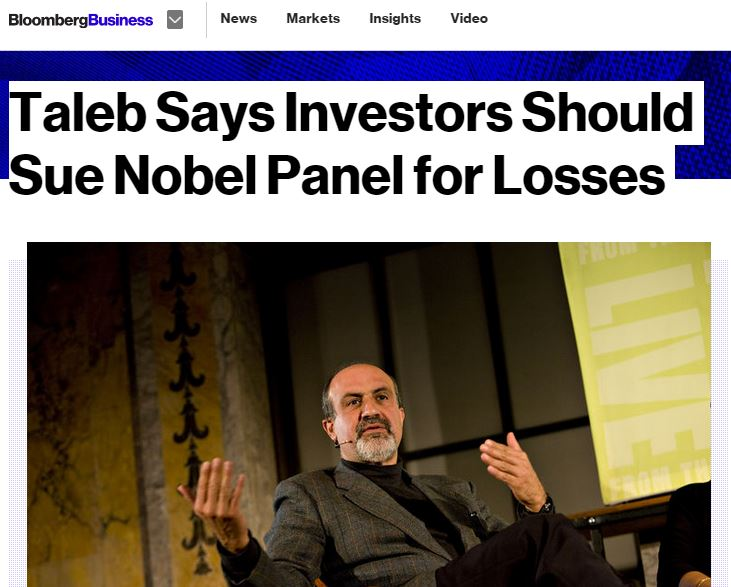
\includegraphics[width=1.05\linewidth]{images/taleb}

\end{figure}

	\end{frame}
%================================================================================ %
	\begin{frame}
\begin{figure}
\centering
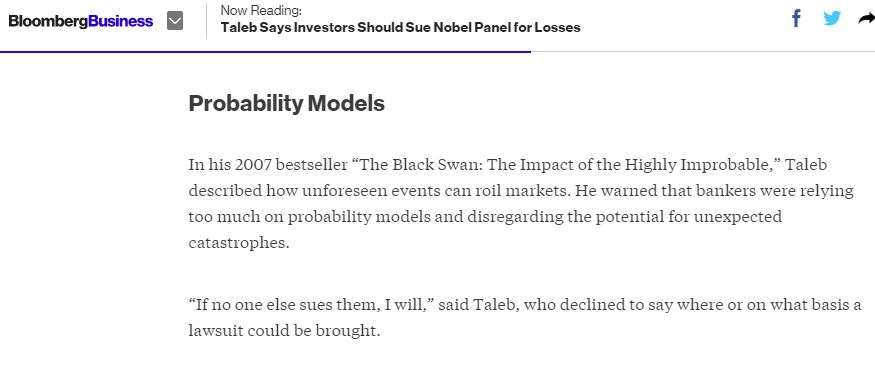
\includegraphics[width=1.05\linewidth]{images/taleb2}

\end{figure}
		
	\end{frame}	
	%============================================================================== %
	\begin{frame}
		\large
	\begin{framed}
		\begin{quote}
	``What goes out of the window? The entire discipline of modern finance and portfolio theory (the theories named after Harry Markowitz, William Sharpe, Merton Miller), the model-based methods of Paul Samuelson, much of time series econometrics (which don’t appear to predict anything), along with papers and theories that are based on “optimization.” These bring fragility into the system."
	\end{quote}
	\end{framed}
	
	(Remark: The basis of his argument in this matter has little to do with his Black Swan Theory).
	\end{frame}
\end{document}